% MIT License

% Copyright (c) 2019 Orange Lee

% Permission is hereby granted, free of charge, to any person obtaining a copy
% of this software and associated documentation files (the "Software"), to deal
% in the Software without restriction, including without limitation the rights
% to use, copy, modify, merge, publish, distribute, sublicense, and/or sell
% copies of the Software, and to permit persons to whom the Software is
% furnished to do so, subject to the following conditions:

% The above copyright notice and this permission notice shall be included in all
% copies or substantial portions of the Software.

% THE SOFTWARE IS PROVIDED "AS IS", WITHOUT WARRANTY OF ANY KIND, EXPRESS OR
% IMPLIED, INCLUDING BUT NOT LIMITED TO THE WARRANTIES OF MERCHANTABILITY,
% FITNESS FOR A PARTICULAR PURPOSE AND NONINFRINGEMENT. IN NO EVENT SHALL THE
% AUTHORS OR COPYRIGHT HOLDERS BE LIABLE FOR ANY CLAIM, DAMAGES OR OTHER
% LIABILITY, WHETHER IN AN ACTION OF CONTRACT, TORT OR OTHERWISE, ARISING FROM,
% OUT OF OR IN CONNECTION WITH THE SOFTWARE OR THE USE OR OTHER DEALINGS IN THE
% SOFTWARE.

\section{XAML 简介}

\subsection{XAML 是什么}

XML(Extensible Markup Language,可扩展标记语言)\index{XML}\index{Extensible Markup Language}\index{可扩展标记语言}
是一种标记语言,用于保存数据。

而 XAML(Extensible Application Markup Language,可扩展应用程序标记语言)\index{XAML}\index{Extensible Application Markup Language}\index{可扩展应用程序标记语言}
也是一种标记语言,并且 XAML 是基于 XML 的。XAML 是微软为构建应用程序用户界面而创建的一种语言。使用它,能让界面的设计与 C++ 等代码分离。\cite{XAMLbaidu}

我们可以看到,在刚才的 Hello World 中,界面对应的 XAML 代码如下。

\begin{lstlisting}[language = xml]
<Page
    x:Class="Hello_World.MainPage"
    xmlns="http://schemas.microsoft.com/winfx/2006/xaml/presentation"
    xmlns:x="http://schemas.microsoft.com/winfx/2006/xaml"
    xmlns:local="using:Hello_World"
    xmlns:d="http://schemas.microsoft.com/expression/blend/2008"
    xmlns:mc="http://schemas.openxmlformats.org/markup-compatibility/2006"
    mc:Ignorable="d"
    Background="{ThemeResource ApplicationPageBackgroundThemeBrush}">

    <Grid>
        <TextBlock HorizontalAlignment="Left" Margin="10,10,0,0" Text="Hello World" TextWrapping="Wrap" VerticalAlignment="Top" FontSize="72"/>

    </Grid>
</Page>
\end{lstlisting}

可以很清楚地看到,刚才从工具箱中拖出来的 TextBlock 变成了一句 XAML 代码,而且这句代码是在一个 Grid 之中的。Grid 的中文翻译为``网格'',顾名思义,使用 Grid 能够将布局分割为网格状,在每个网格中可以再形成一个布局。在 Hello World 中,我们实际上是在一个 Grid 的唯一一个网格中放置了一个 TextBlock。

\subsection{为什么要使用 XAML}

好处之一在前面已经提到过,XAML 的存在让我们能够将界面与 C++ 代码分离,便于分工。另一个好处是,从上面也可以看出,XAML 比较适合描述界面这种层次性的结构。

\subsection{小试身手:让我们的 TextBlock 居中显示}

尝试如下代码代替上面的 TextBlock:
\begin{lstlisting}[language = xml]
    <TextBlock Text="Hello World" FontSize="72" HorizontalAlignment="Center" VerticalAlignment="Center"/>
\end{lstlisting}

见图 \ref{pic14},我们对代码的修改可以实时通过可视化编辑器体现出来。
\begin{figure}[htbp]
    \centering
    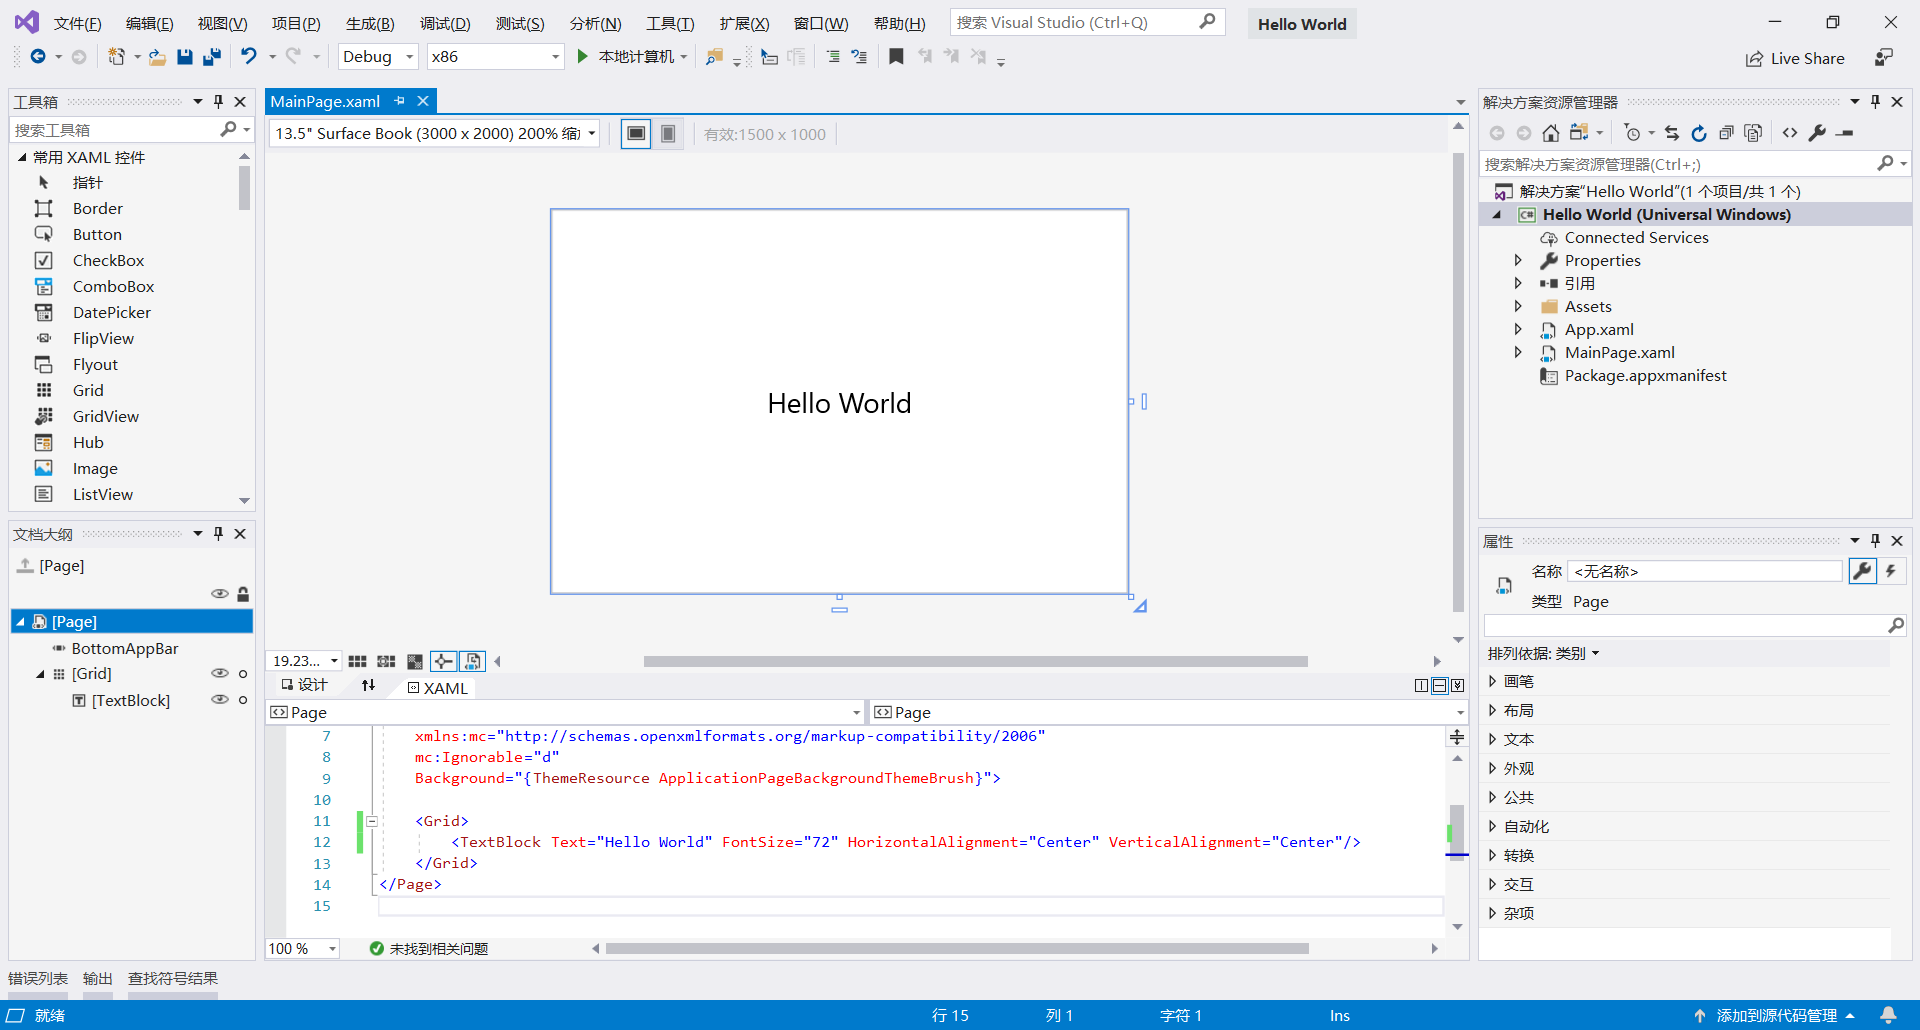
\includegraphics[width = 0.75\paperwidth]{pic/14.png}
    \label{pic14}
    \caption{通过可视化编辑器实时预览对 XAML 代码的修改。}
\end{figure}

我们在什么都不会的情况下,通过对已有代码的简单模仿,成功做到了让 TextBlock 居中显示,可见 XAML 是很好上手的。